\section{Introduction}

\subsection{Adaptive mutations}

Biologists have long wondered the extent to which evolution occurs due
to nearly neutral and slighly deleterious mutations, or adaptive
mutations, or more complex situations involving these types of
mutations as well as their epistatic interactions (cite the work of
Kimura etc.).

The occurence of beneficial mutations and how they affect adaptation
is currently an area of active interest in evolutionary biology
\citep{Chou2011, Weinreich2006}. Although much focus in the past
has been placed on deleterious mutations because of their prevalence
in nature and disease, it is ultimately beneficial mutations that
are responsible for adaptive evolution.
 
\subsection{Adaptive mutations and epistasis}


Since beneficial mutations are relatively rare, and since
combining multiple mutants in the lab is increasingly difficult for
the more mutations that are to be combined, an \textit{in silico}
analysis can shed light on what may be expected in adaptive
evolution.



\subsection{The need for a new modeling framework}
Clearly, using FBA with the growth objective alone is not enough--we
only ever get the optimum for our fitness objective.  A way to
circumvent this issue is to associate a feature of the system
(e.g. flux into biomass) as the fitness while optimizing some other
objective. This latter mechanism is not generally used as most models
tend to be rather under-constrained as is. However, as we've seen, the
FALCON method 
\ifthenelse{\boolean{thesisStyle}}{(Chapter~\ref{chap:FALCON})}{} 
and other fitting methods like MoMA provide a
way to use high-throughput data to introduce many additional
constraints to the system.

Having a systems tool that can work with models of particular organisms
will not only add another tool in the computational evolution and
population genetics arsenal, but also in applied fields such as
evolutionary engineering of microbial engineering, and understanding
which gene mutant combinations which may be most advantageous for
a cancer cell population.

\section{Results}

\subsection{Weighted MoMA-FBA objectives}

Minimization of metabolic adjustment (MoMA), along with Flux Balance
Analysis (FBA), has proven successful in simulating growth rates and
predicting in silico fluxes. Here we discuss a weighted objective
approach that combines both objectives. 

The typical MoMA problem is framed as a least-squares optimization
problem and is typically employed to calculate the flux vector of an
\emph{in silico} organism after a mutation \cite{Segre2002_sb2013}.
The biological intuition is that the organism has not had time to
adapt to the restricted metabolic capacity and will maintain a similar
flux to the wild-type (WT). If $\mathbf{a}$ is the WT flux vector
obtained by an optimization procedure, such as min-norm FBA (flux
balance analysis), then in a model with $N$ reactions the optimization
objective can be expressed as
\[ \textnormal{minimize}\ \sum^N_{i=1}(v_i-a_i)^2 \] 
subject to the stoichiometric constraints $\mathbf{S_{int} v} =
\mathbf{0}$ where $\mathbf{S_{int}}$ is composed of rows in the
stoichiometric matrix involving internal metabolites and $\mathbf{v} =
(v_1, \ldots, v_N)^T$.  Additional constant bounds on fluxes are often
present, such as substrate uptake limits, so we write $\mathbf{v}_{lb}
\preceq \mathbf{v} \preceq \mathbf{v}_{ub}$. The objective may be
equivalently expressed in the canonical quadratic programming (QP)
form
\[ \textnormal{minimize}\ \frac{1}{2}\mathbf{x}^T \mathbf{Q x} + \mathbf{c}^T \mathbf{x}\]
as  
\[ \textnormal{minimize}\ \frac{1}{2}\mathbf{v}^T \mathbf{v} - \mathbf{a}^T \mathbf{v}\textnormal{.}\]

When we try the standard MoMA procedure in a new environment, several
things become clear. For instance, switching the energy and carbon
source from glucose to ethanol will result in zero growth because the
biomass is relatively small compared to other fluxes numerically.
This is easily fixed by adding a weight to the biomass, though there
are also certain numerical issues related to this with at least some
solvers (e.g. MOSEK) that require an inverse weight on all other
fluxes.

To accomodate these weights, let $w$ be a positive scalar weight, and
let $f(w)$ and $g(w)$ be two scalar weight functions such that $f(w) >
0$ and $g(w) > 0$ for all $w \ge 1$. We also assume $f(w)$ is
monotonically increasing and $g(w)$ is monotonically decreasing. While
$g(w)$ is employed to achieve the inverse weighting mentioned above,
$f(w)$ is used to achieve gradual regularization as $w$
increases. Biologically, regularization is important as it allows
efficiency in enzyme synthesis to be modeled, which is typically done
in FBA by requiring a min-norm flux.  We incorporate these weights
into the objective:

\[ \textnormal{minimize}\ \sum^N_{i=1,i\ne b}g(w)(v_i-a_i)^2 - w v_b + \sum^N_{i=1,i\ne b}f(w)v^2_i \]

Index $b$ corresponds to the growth or biomass pseudo-reaction.  In
the simulations below, $g(w) = \frac{1}{\sqrt{w}}$. For some
simulations we haven't yet used a nonzero $f(w)$, but an example we
have used is $f(w) = \frac{\log{(\log{w}+1)}}{C}$ where $C$ is a
scaling constant.

% \footnote{We
% typically also incorporate shadow prices, see section XXXX.}
  
Express this objective as

\[ \textnormal{minimize}\ \frac{1}{2}\mathbf{v}^T \mathbf{Q v} - \tilde{\mathbf{a}}^T \mathbf{v}\]

where $b = N$ for convenience, $\tilde{\mathbf{a}} = g(w)\mathbf{a}$
with the Nth entry replaced by $w$, and

\[ \mathbf{Q} = \begin{pmatrix}
f(w)+g(w) & 0       & \cdots    & 0 \\
0         & \ddots  & 0         & \vdots \\
\vdots    & 0       & f(w)+g(w) & 0 \\
0         & \cdots  & 0         & 0  
\end{pmatrix}\textnormal{.}\]

For convenience, informally denote this objective function as
$\mathcal{M}(w,d_1,\dots,d_m)$ where the optional $d_i$ represent
possible mutations to the model.

The difference in smoothness between weighted quadratic MoMA and linear
MoMA can be illustrated by considering the growth rate to be a
function of the weight placed on the biomass objective
(\Fig~\ref{fig:Fitness_LM_QP}).  An advantage of quadratic MoMA is
that it simulates a continuous range of fitnesses 
potentially matching any required fitness level exactly.  Quadratic
programming does not admit alternative optima either, if the objective
is convex, as in MoMA. However, these benefits are not necessarily
always biologically relevant; discrete mutations may give a discrete
jump in fitness. There is no obvious reason why having a unique optima
would be biologically preferred; in fact, when compared to simple
objectives like MoMA or FBA, most biological systems appear to operate
suboptimally \citep{Schuetz2012}. Weighted linear MoMA can model these
discrete transitions in flux state, and often this is reflected in
discrete jumps in fitness, as seen above.

\begin{figure}
\centering
  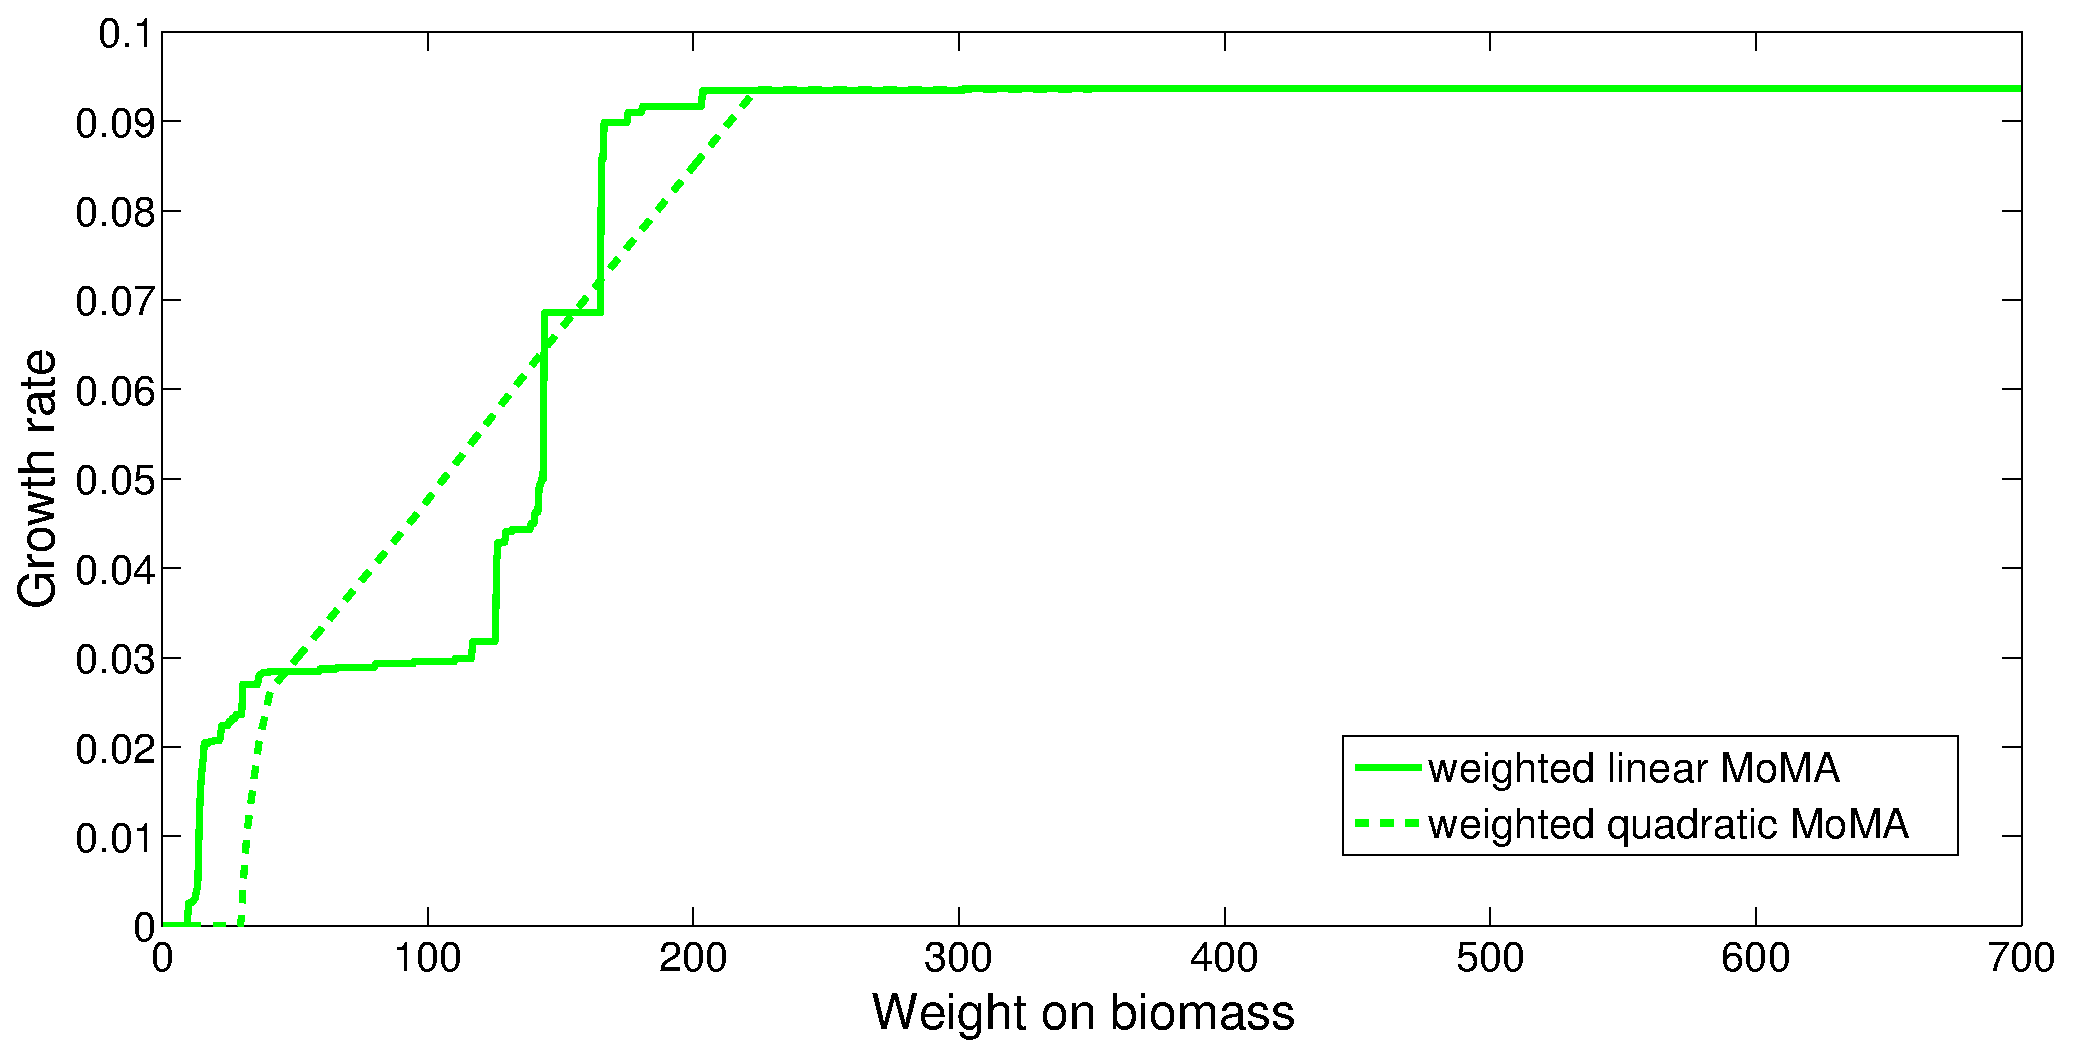
\includegraphics[width=\textwidth]{Fitness_LM_QP}
  \caption{Weight on the biomass component of an objective (x-axis)
  influences the growth rate, where the other objective component is a
  MoMA objective that tries to minimize the flux difference with an
  ancestral environment.}
  \label{fig:Fitness_LM_QP}
\end{figure}

In the above figure, the difference in fitness between weighted
quadratic MoMA and linear MoMA can be seen. An advantage of quadratic
MoMA is that it simulates a continuous range of fitnesses, potentially
matching any required fitness level exactly.  However, this is not
necessarily always biologically relevant; in reality, discrete mutations may give
a discrete jump in fitness. Weighted linear MoMA models these discrete
transitions in flux state, and often this is reflected in discrete
jumps in fitness, as seen above.

\subsubsection{Weighted MoMA predicts expression states}

Using tiling array data for s288c in YPD and YPE conditions from
\citet{Xu2009}, we compare the number of genes expected to have a
two-fold or greater change in expression from YPD to YPE to the fluxes
mapped to genes also having greater than two-fold change in the same
environmental transition. The x-axis represents the weight on
growth. The number of
genes having more than two-fold flux and expression change in the model and and
in the experiment are shown in blue. The red and red dotted lines
represent the random expectation and 95\% CI for expression agreement
for a random expression vector with the genes belonging to the model
and experimental dataset. The random expression vector has the same
number of two-fold up-regulated and two-fold down-regulated genes as the
real relative expression vector.

\begin{figure}
\centering
\begin{tabular}{c}
\begin{subfigure}[b]{\textwidth}
  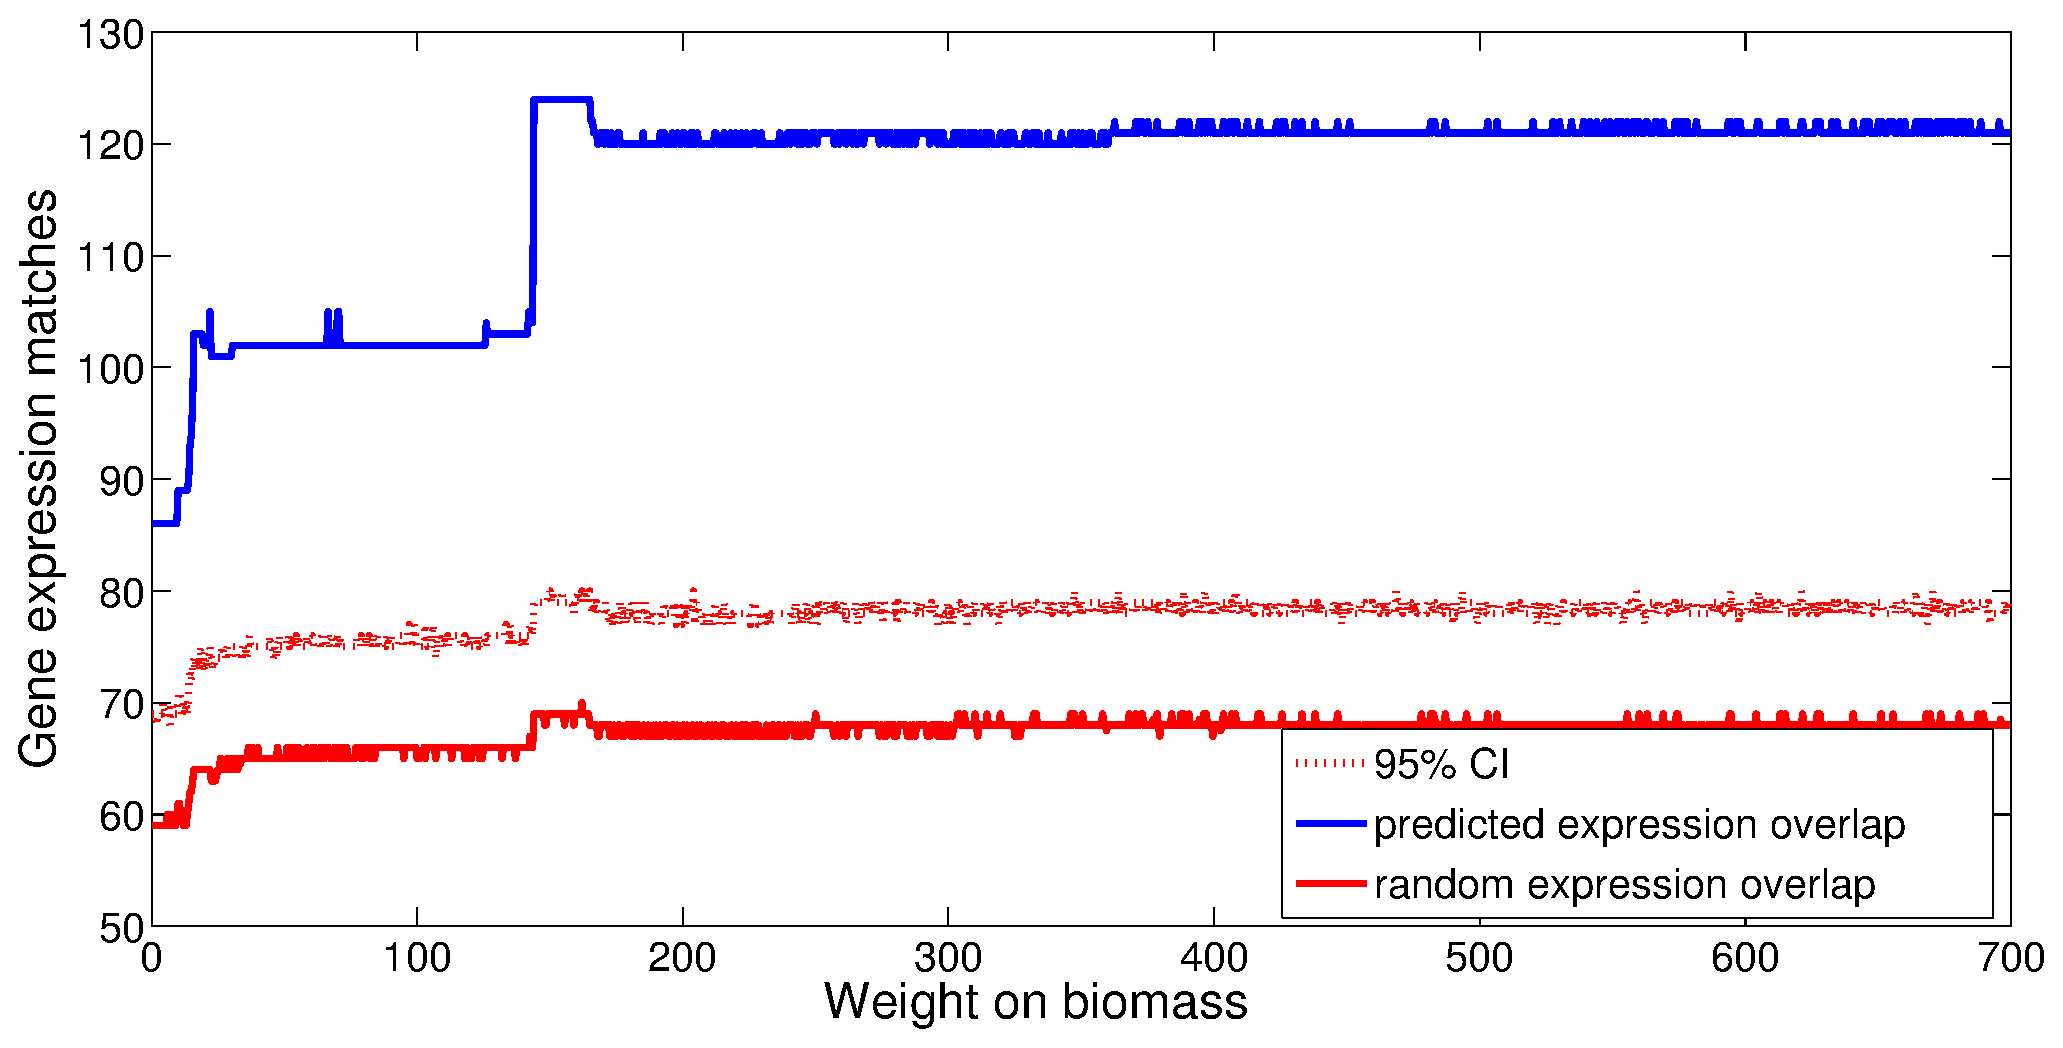
\includegraphics[width=\textwidth]{randGene_noFit}
  \caption{Linear MoMA} 
  \label{fig:randGene_noFit}
\end{subfigure}
\\
\begin{subfigure}[b]{\textwidth}
  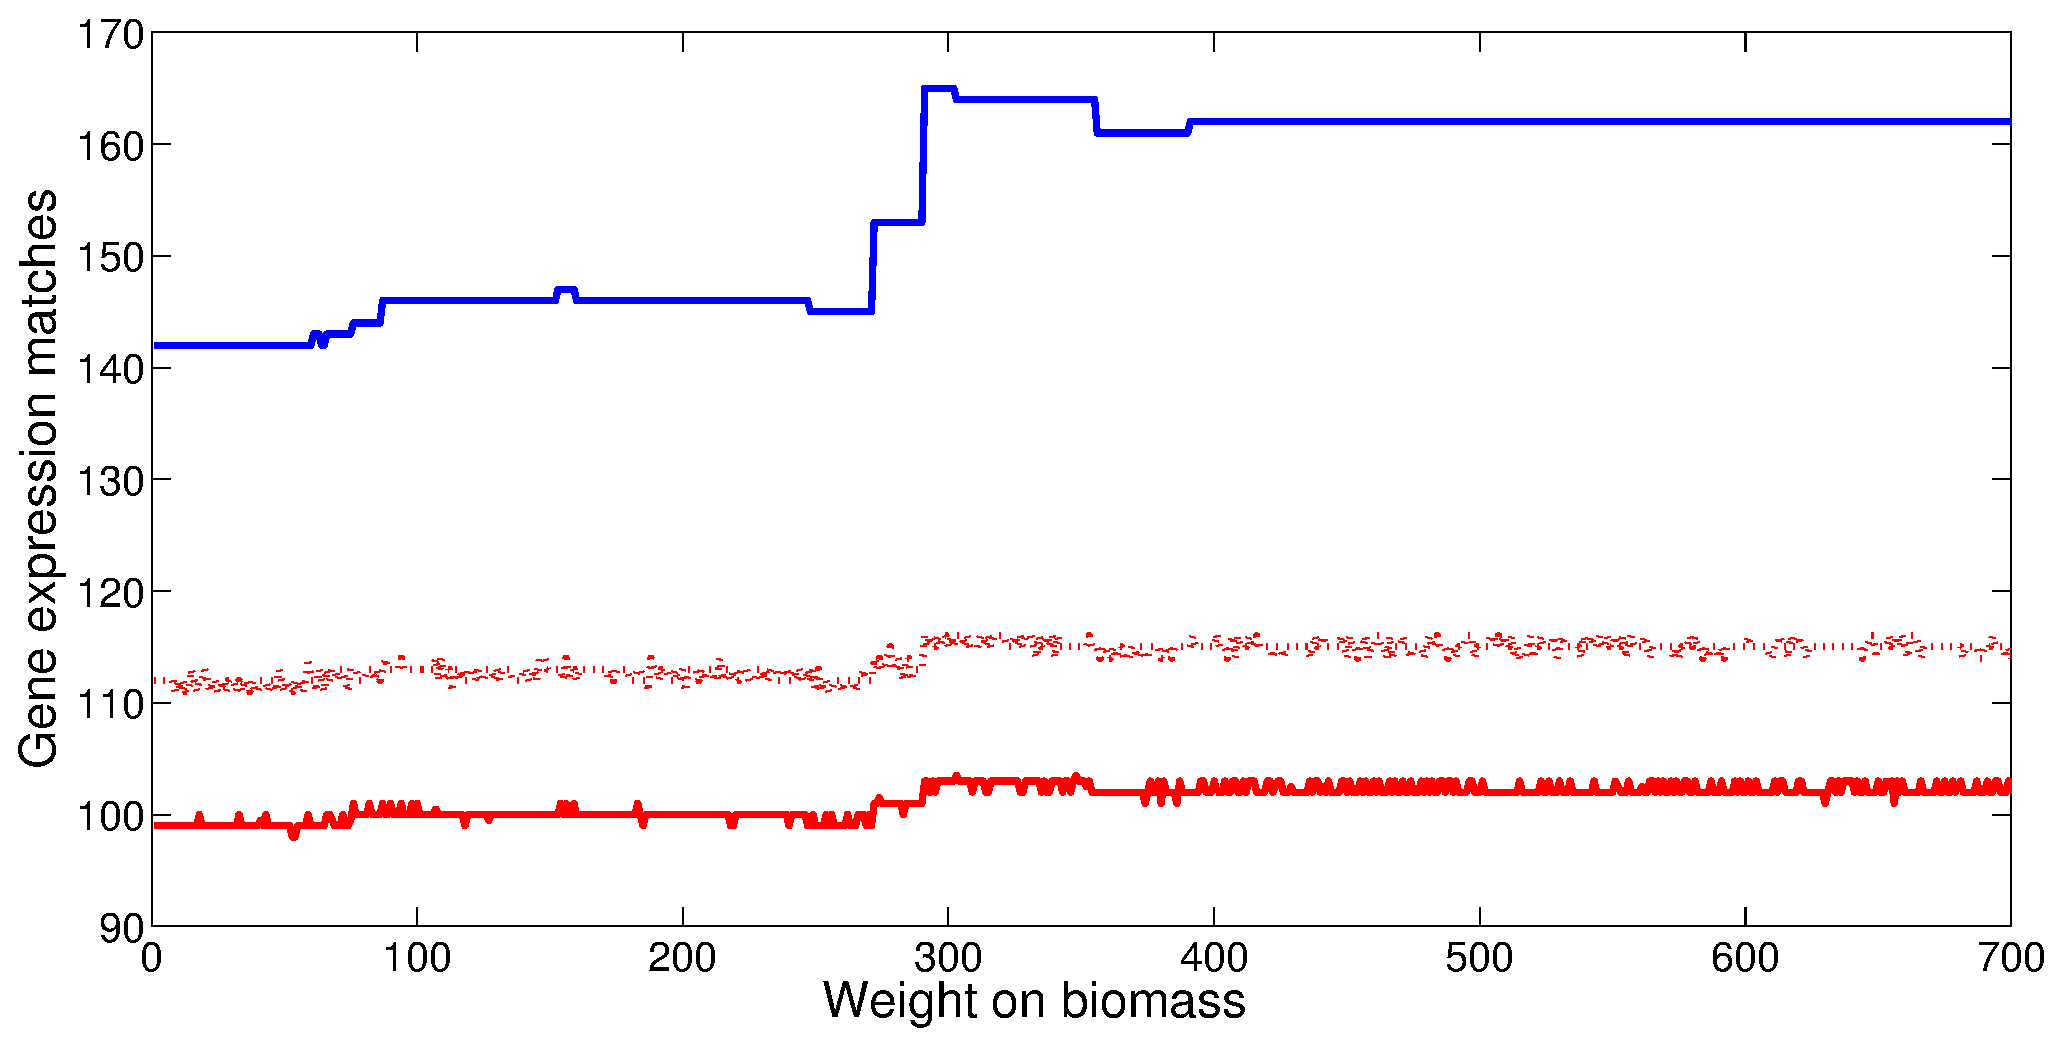
\includegraphics[width=\textwidth]{randGene_noFit_QP}
  \caption{Quadratic MoMA} 
  \label{fig:randGene_noFit_QP}
\end{subfigure}
\\
\end{tabular}
\caption{Number of yeast genes that are at least two-fold up-regulated
or down-regulated when going from YPD to YPE media with matching
predictions from weighted MoMA (blue line) and the associated 95\%
confidence interval (red dotted line) around the prediction to random
chance (red line).}
\label{fig:wMoMA_expMatch}
\end{figure}


Interestingly, the weight and corresponding fitness that agrees most
with the experimental predictions is sub-optimal in both the quadratic
and linear cases, suggesting that the s288c strain was not fully
adapted to the YPE environment when the expression was assayed.  To
compare directly with geometric FBA (a minimal $\textbf{\textit{L}}^1$-norm solution), we found
that geometric FBA had 123 concurring genes whereas weighted linear
MoMA had 124; similarly, a minimal $\textbf{\textit{L}}^2$-norm FBA solution in Ethanol had 162
agreeing solutions and weighted quadratic MoMA had 165, showing that
weighted MoMA can do at least as good as the gold standards for \textit{de
novo} FBA solutions in predicting accurate fluxes.


\subsubsection{Simulated adaptation induces complexity in sub-optimal solutions}

Previous work explored the complexity of optimal and sub-optimal flux
vectors, finding that generally the sub-optimal solutions have more
active fluxes than the optimal solutions \citep{SangLee2012}. We found
a similar trend with weighted MoMA where, once growth is non-zero, the initial flux state
has more active reactions than in the ancestral environment (glucose;
red dashed line) or than in the more adapted stages in the current
(ethanol) environment (\Fig~\ref{fig:complexityEth}).


\begin{figure}
\centering
  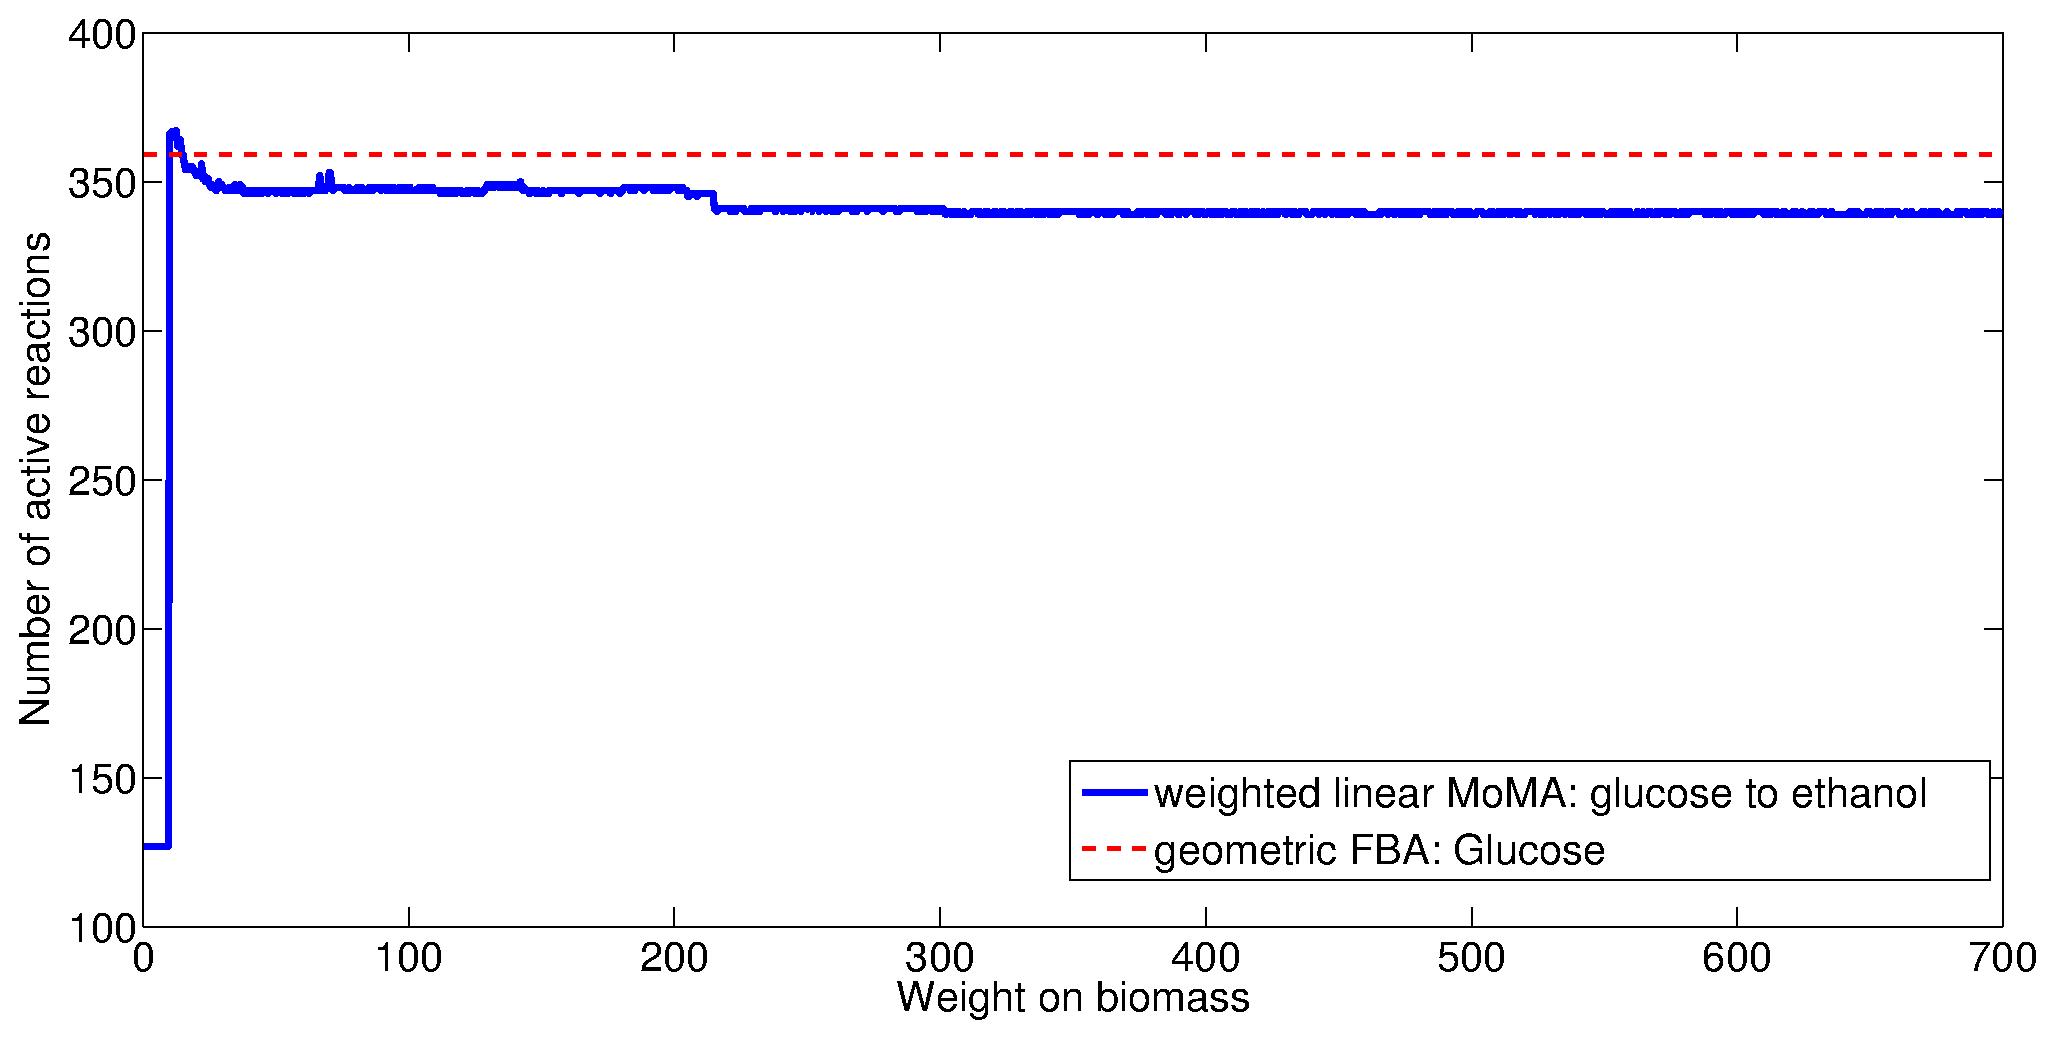
\includegraphics[width=\textwidth]{complexityEth}
  \caption{The number of active reactions (reactions with non-zero
  flux) plotted against the weight on the biomass component of a
  weighted linear MoMA objective (blue). An flux that maximizes biomass
  production that is centered among alternative optima is shown for
  comparison (red dotted line).}
  \label{fig:complexityEth}
\end{figure}


\subsection{Adaptive mutations with objective weights}

Aside from the problem of separating the fitness function from the 
optimization objective function, there is the issue of combining traditional flux
restriction mutations, which are known as \emph{hard constraints}, which may
result in an unsolvable system --- an almost certainly undesirable
effect of this mutation modeling formalism. Instead, it would be
better if mutations could be modeled as \emph{soft
  constraints}. Concretely, whereas hard constraints are enacted in
the actual constraints of the optimization problem, soft constraints
merely change the objective. This means that multiple soft constaints
combined together under some mutational model would be compatible in
the sense that they wouldn't unexpectedly result in an unsolvable
system. When performing growth optimization in FBA, normally only the
biomass pseudo-reaction has a non-zero (positive) entry. Nonzero
values for any other entry could only decrease the flux. In weighted
MoMA or FALCON, nonzero coefficients for any enzymatic reaction could
prove potentially beneficial, as they may push the system in a
direction that is more in line with growth optimization and less in
line with MoMA or the FALCON flux-fitting objective.

FALCON and weighted MoMA provide two possible avenues for soft constraints:
expression level and expression variation. However, it is not clear
yet what expression variation really means, so further investigation
is necessary. Furthermore, using a hard constraint model for mutants,
as opposed to a soft constraint like weights on fluxes, appears to
reduce the amount of non-trivial interactions: in the hard-constraint
method one highly beneficial mutation may exactly subsume the mutation
of a less beneficial mutant by forcing flux through the reaction; this
happens to a certain extent in the weighted model as well, but not
nearly as frequently.

An example for both the quadratic and linear cases exemplifies the
difference in smoothness obtained from using either a linear or
quadratic objective for weighted MoMA with objective weights (mutations)
on a particular reaction (\Fig~\ref{fig:wMoMA_smoothness}).


\subsection{Adaptive trajectories and evolutionary path analysis}

Phenotypes involving a small number of mutations have had their
adaptive paths analyzed systematically (\citep{Poelwijk2007,Weinreich2006, 
Khan2011, Chou2011}; four or five mutations). In \citet{Weinreich2006}, all
mutations occur on a single enzyme, and even in such a localized case,
sign epistasis, which gives rise to evolutionary traps, occurs for the
majority of mutational paths. In the present study, we used less
severe grounds for deciding if an evolutionary path is a likely
dead-end, but even so, we can see that (\Fig~\ref{fig:trapAnalysis};
\suppOrApp Section~\ref{sec:pathAnalysis}).

\captionpage{figure}{%
An examination of simulated evolutionary dead-ends. Randomly selecting
10 beneficial mutations from over 150 total benefical mutations in a
yeast model will have a varying number of mutations that are present
in the combinatorial mutant with the highest fitness The percent of
paths that reach the optimal mutant by avoid traps tends to decrease
as more mutations are considered (\ref{fig:trapAnalysis:percPath}), or
viewed another way, the mean number of paths stopped by traps tends to
increase (\ref{fig:trapAnalysis:meanStop}).}
\label{fig:trapAnalysis}

\begin{figure}[H]
\newlength{\figwidth}
\setlength{\figwidth}{0.9\textwidth}
\centering
\begin{tabular}{c}
\begin{subfigure}[b]{\figwidth}
  \includegraphics[width=\textwidth]{percNoTrap_tmp}
  \caption{}
  \label{fig:trapAnalysis:percPath}
\end{subfigure}
\\
\begin{subfigure}[b]{\figwidth}
  \includegraphics[width=\textwidth]{trapMeanStop_tmp}
  \caption{} 
  \label{fig:trapAnalysis:meanStop}
\end{subfigure}
\\
\end{tabular}
\end{figure}


In a genome-scale metabolic model, we observe that while the majority
of paths are not likely to have a problem, once eight or nine genes are
involved, the average number of paths to reach the optimum without
experiencing a trap are only ~65\%. This demonstrates that the
presence of traps are heterogeneous, just as in the single-enzyme
experiment of \citet{Weinreich2006}, suggesting that the order of
mutations often matter to a very significant degree in evolution.

The fact that many unobstructed evolutionary paths are observed at the
genome-scale suggests that evolution is, in general, not very
predictable (\Fig~\ref{fig:trapAnalysis}). However, if we consider
that neutral mutations are unlikely to fix in a population, the number
of viable paths would greatly decrease (\suppOrApp
Section~\ref{sec:pathAnalysis}). Interestingly, in every experimental
case (Table~\ref{tab:threeAdaptEvoDats}), only a single fitness peak
appears to be present \citep{Lunzer2005,Weinreich2006}. When we
consider simulations from
genome-scale models instead of isolated pathways or single protein, we
still observe the single fitness optima for five mutation sets, but
once we consider eight mutations, every set of eight or more mutations
presents with multiple local optima. This suggests that evolution
becomes not only less predictable when we look at evolution of larger
systems or evolution at a large time scale, but also less likely to
reach the global optimal fitness.


\subsubsection{Software for evolutionary path analysis}

Storing all evolutionary paths in memory or disk can become 
intractable. For instance, even 10 mutations has $10! \approx
3.6$ million possible paths, but only $2^{10} = 1,024$ mutant
combinations. Due to this difficulty, we have created software to allow 
the dynamic exploration and analyses of these paths. 

The C programs for dynnamically performing analyses on text files
containing fitness data for all combinations of $n$ mutations can be
found online, and additional information and and examples related to
usage is available (\suppOrApp Section~\ref{sec:pathAnalysis}).

\subsubsection{Small beneficial mutants exhibit positive epistasis}

Prior studies using metabolic models have shown that deleterious
mutations tend to exhibit negative epistasis for stronger mutations
and positive epistasis for weaker mutations (\citep{He2010, Xu2012};
\hl{add full figure from MS1}). The reason for positive epistasis
being prevalent for deleterious mutations is that most of them occur
in essential pathways, and one mutation will buffer against the
effects of a second mutation (\citep{Xu2012}). Somewhat surprisingly,
we also see that predictions for epistasis involving weakly beneficial
mutations also tend to have positive epistasis
(\Fig~\ref{fig:beneEpiPairwise}; Section~\ref{sec:falconLMoMAEpistasis}). 
This trend is verified for two experiments involving
multiple genes (as in our simulation) where fitnesses are readily
calculated (\citep{Chou2011, Khan2011}; Table~\ref{tab:pairwiseBeneEpi}).

\begin{table}
\newcommand{\hlB}{\cellcolor{blue!20}}
\newcommand{\hlR}{\cellcolor{red!20}}
\centering
\begin{tabular}{cc}
\begin{subtable}[b]{0.5\textwidth}
\caption{\citet{Khan2011}}
\begin{tabular}{cccccc}
fitness &   & t           & s           & g           & r           \\
1.145   & t &             &             &             &             \\
1.108   & s & \hlB -0.060 &             &             &             \\
1.030   & g & \hlB -0.027 & \hlB -0.014 &             &             \\
1.015   & r & \hlB -0.056 & \hlB -0.004 & \hlR 0.005  &             \\
1.003   & p & \hlR  0.049 & \hlR  0.078 & \hlR 0.045  & \hlR 0.007  \\
\end{tabular}
\end{subtable}
&
\begin{subtable}[b]{0.5\textwidth}
\caption{\citet{Chou2011}}
\begin{tabular}{ccccc}
fitness &       & gshA        & GB          & fgh         \\
1.509   & gshA  &             &             &             \\
1.166   & GB    & \hlB -0.120 &             &             \\
1.142   & fgh   & \hlB -0.100 & \hlB -0.012 &             \\
1.096   & pntAB & \hlB -0.040 & \hlR  0.021 & \hlR 0.029  \\
\end{tabular}
\end{subtable}
\\
\end{tabular}
\caption{Pairwise epistasis values (calculated multiplicatively) from 
two experimental systems. \hl{Need to describe mutations and systems}.}
\label{tab:pairwiseBeneEpi}
\end{table}


The trend for increasing negative epistasis as mutations become
increasingly beneficial (also termed \textit{diminishing returns
epistasis}; \citep{Chou2011}) can be easily understood in most
contexts, including metabolism, due to the fact that in any given
environment there must be a physiological maximum value for most
phenotypes, including growth rate of a cell or individual organism.
Thus, if one mutant is extremely beneficial, it proportionally limits
the effect another beneficial mutant might have when combined
together. Such decreasing marginal benefits are not the only reason we
may tend to see small mutants with positive epistasis; Fisher's
geometric model implies that increasing complexity will decrease the
likelihood that any given mutation will be beneficial, and
increasingly so for mutations with more extreme changes in the
phenotypic space \citep{Orr2000}. Since a mutation that exhibits
positive epistasis with many other mutations is just a way of saying
the mutation is likely to be beneficial on many genetic backgrounds,
the effect observed by \citet{Orr2000} extends beyond absolute fitness
values and into the epistatic landscape. Furthermore, in our
metabolic models (as in most biological systems), fluxes do not
operate in isolation; a mutation in a gene expression level or
reaction constraint will affect other reaction fluxes in the system,
and can be classified as pluripotent. If it is an essential reaction,
many fluxes are likely to be affected, thus exhibiting a complex
phenotype and a high degree of pluripotency. Large pluripotent
mutations would then be expected to have a larger total length in
Fisher's geometric model, and be less likely to be beneficial or have
positive epistasis.  This is exactly what we see in metabolic models
with deleterious mutations, which tends to exhibit positive epistasis
for smaller mutations and negative epistasis for more extreme
mutations (\hl{cite suppl grid fig}; \citep{He2010, Xu2012}).


This trend in epistasis can also be captured by our constraint-based
modeling framework for beneficial mutations. After \textit{in silico}
screening for beneficial mutations
(Section~\ref{sec:epiBeneMethodSS}), we can examine trends in
pairwise epistasis as a function of the single mutant fitnesses 
\Fig~\ref{fig:beneEpiPairwise}. A fairly distinct border appears
to be present between the region that has some positive epistasis and
no positive epistasis. By considering that an epistatic cutoff (call
it $\epsilon_c$) is employed, we may use the multiplicative epistatic
relationship $W_{xy} - W_x W_y > \epsilon_c$, which yields the
reciprocal function $W_y > \frac{W_{xy} - \epsilon_c}{W_x}$ for fixed
$W_{xy}$, which limits the region in which positive epistasis, as
defined by $\epsilon_c$, can occur. Since $W_{xy}$ is not a constant,
there may be some variation in the actual trend from a true reciprocal
function.

%Change to two col later?
\begin{figure}
\centering
\begin{tabular}{c}
\begin{subfigure}[b]{\textwidth}
  \includegraphics[width=\textwidth]{beneEpiMean_tmp}
  \caption{mean epistasis} 
  \label{fig:beneEpiPairwise:mean}
\end{subfigure}
\\
\begin{subfigure}[b]{\textwidth}
  \includegraphics[width=\textwidth]{beneEpiPerc_tmp}
  \caption{percent of positive epistasis}
  \label{fig:beneEpiPairwise:perc}
\end{subfigure}
\\
\end{tabular}
\caption{The mean epistasis (\ref{fig:beneEpiPairwise:mean}) and percentage
  (\ref{fig:beneEpiPairwise:perc}) of positive epistasis for epistases such
  that $\left|\epsilon\right| \ge 0.01$.}
\label{fig:beneEpiPairwise}
\end{figure}

The distribution of epistases arising from beneficial mutations is
highly similar to that found in natural biological systems that are
also described by population genetic models
(\Fig~\ref{fig:epiBeneDist}; \citep{Martin2007a}). Interestingly, the
small-scale data from \citet{Martin2007a} is from an RNA virus (VSV),
whereas our stoichiometric models are not designed for modeling
viruses. Nonetheless, the trend remains similar, suggesting that this
is a trend that extends across completely different types of models as
well as from the fitness of complex life forms and simple non-living
viruses. This excellent fit requires that an appropriate distribution
of fitnesses is sampled according to extreme value theory (EVA;
Section~\ref{sec:epiBeneMethodSS}; \citep{Orr2005, Orr2003}).


\begin{figure}
\centering
  \includegraphics[width=\textwidth]{99p9_epi_YPD_tmp}
  \caption{Distribution of epistases arising in a yeast model from
beneficial mutations sampled according to EVA.}
  \label{fig:epiBeneDist}
\end{figure}

\section{Discussion}

We have developed a data-driven modeling framework in the
constraint-based metabolic modeling family that allows the exploration
of combinatorial epistases and reproduces trends seen from studies in
the forefront of evolutionary research \citep{Martin2007a, Chou2011,
Khan2011}. Contemporaneous, theoretical insights in to how a general
clas of mechanistic models, encompassing those used in this study,
give rise to traditional population genetic models such as Fisher's
geometric model \citep{Martin2014}.  The methodologies described in
this paper should have applications in diverse fields due to their
reliance on mechanistic models available for many organisms
\citep{Monk}.

The questions are often
difficult or impossible to assess experimentally due to limited
resources.  In genome-scale models, to our knowledge, only microbial
epistasis has so far been studied for all enzymes (often referred to
as genome-scale in this context). This is due to several factors.

One issue is that these computations can still take a significant
amount of time, and the increase in model size of Human Recon 2 over
Yeast can cause even a relatively simple FBA run to go up by an order
of magnitude.  This problem is compounded by the increase in the
number of genes in the human model, since computing epistasis consumes
space and time as $O(n^2)$ where $n$ is the number of genes in the
model. More important than this issue, which might be overcome with
enough computational resources, is the issue of an objective
function. It has been shown numerous times that FBA with a biomass
objective can be a reasonable approximation to what a microbe is
trying to achieve metabolically
\citep{Schuetz2012, Fong2004, Varma1994}. While Recon 2
is equipped with a ``generalized biomass reaction'', it is not clear
what the meaning of this is, and it certainly seems to greatly overestimate
the metabolism even of fast-growing cancer cells \citep{Mehrara2009}.
We propose FALCON as a potential method to get around this issue
for non-microbial models.

Another advantage of FALCON is that it allows one to directly probe
mutations that are represented as gene expresion perturbations. A
decreased level of gene expression may also be metabolically
equivalent to the effect of a missense mutation, for example. This
allows a different sampling strategy than before; for instance, we
could observe how uniform expression restriction compares to uniform
flux restriction~\citep{Xu2012}. Assuming an accurate model of
enzyme-complex expression measurement, the former should be the more
realistic model.

A limitation is that we have only considered metabolic genes and their
effect on steady-state metabolism. While in principle a similar method
could be applied to whole cell models \citep{Karr2012, O'Brien2013}, the
computation time would not be feasible to the screening for beneficial
muatations, nor of exploring them combinatorally, as the time needed
for a single mutant takes at least a day even in the smallest
bacterial model \citep{Karr2012}. Future isnights into improving the
efficiency of whole cell models, or making a compromise on which
systems are simulated (e.g. rFBA, \citep{Covert2001}), may improve
these efforts.

\section{Methods}
\label{sec:epiBeneMethod}
%
% Some defs
%
\newcommand{\FVAmin}{F_{\textnormal{min}}}
\newcommand{\FVAmax}{F_{\textnormal{max}}}

\subsection{Beneficial mutation simulation for pairwise epistasis}
\label{sec:falconLMoMAEpistasis}
In order to generate a realistic WT flux, we use experimental
expression data to fit a flux vector (\hl{cite falcon and
Lee2012}). Because even FALCON can take one or two orders of magnitude
longer than MoMA (or linear MoMA), we use linear MoMA to estimate the
flux vectors for single and double mutants. Since our fitness is just
flux through the biomass pseudo-reaction, which is a complicated sink,
it never seems to carry a flux in practice when expression-flux
fitting techniques are used. Therefore, we used experimentally
determined growth rates as a constraint in the flux fitting step for
calculation of the WT flux vector \hl{cite these}. Though this
approach was only used for pairwise epistasis in the current study, it
would also be appropriate for combinatorial epistasis (we simply used
FBA to generate wild-type adapted flux vectors for our combinatorial
epistasis simulations).


\subsection{Mutation screening and sampling}
\label{sec:epiBeneMethodSS}

To more closely follow existing theory in population genetics, in
addition to performing uniform sampling of allele phenotypes (\hl{first
figure below; same as previous figures}), we also performed Gaussian
sampling centered at the WT phenotype. For each reaction, we sampled
flux restrictions where the WT flux ($F_{WT}$) was at the mean of the
Gaussian distribution. Since there is some uncertainty in the
underlying distribution of mutational effects that would best reflect
nature, we used several different distributions and employed the FVA
to bound the distribution \citep{Muller2013}. For example, for the
99\% Gaussian sampling below, for each reaction, we sampled fluxes
from a truncated normal distribution between the FVA minimum
($\FVAmin$) and FVA maximum ($\FVAmax$) where the underlying normal
distribution would have 99\% of its density in $F_{WT} \pm
\textnormal{max}\left( \left|F_{WT}-\FVAmin\right|,
\left|F_{WT}-\FVAmin\right|\right)$. This sampling technique (in
particular the symmetric bounds about $F_{WT}$) was chosen in order to
approximate how sampling mutations from Fisher's geometric model
results in a beneficial mutation distribution distribution conforming
to extreme value distributions \citep{Orr2005, Orr2006}. Only
beneficial mutants were kept for the present analysis.

A 99\% sampling strategy will be less likely to sample extremely
divergent fluxes than a 50\% sampling strategy since the tails of the
distribution will be placed further away from the WT in the latter
case. We find it is preferable to sample a high percentage of mutations
that are closer to the WT in order to generate a beneficial
mutation distribution conforming to extreme value theory, since otherwise
the mutation sampling in our metabolic model begins to approximate
a uniform distribution (\hl{\suppOrApp \Fig~\ref{}}).  It can be
seen that epistasis distributions resulting from EVA-conforming
fitness distributions result in a skew toward near-zero epistasis and
positive epistasis as we tend to sample more mutants near the WT
(\Fig~\ref{fig:epiBeneDist}).


%%% TODO %%%

% need more background

% actually try to use FALCON for GxG interactions, discuss caveat
% that it is possible that influencing one enzymatic gene's abundance
% could affect another enzymatic gene's abundance, and we can't directly
% take this into account in our model

% discuss C software a bit more in supplement


% briefly discuss FBA weight possibility as it relates to FALCON

% Discuss sign epistasis (and understand it) more:
% Notes: See Weinreich 2007 for really nice discussion and refs:
% http://webpub.brown.edu/Research/Weinreich/WeinreichPublications/Poelwijk_etal2007.pdf
% http://onlinelibrary.wiley.com/doi/10.1111/j.0014-3820.2005.tb01768.x/pdf
% Note: also discuss the trends found for sign epistasis, if any, in the two recent science papers:
% Khan et al.
% Chou et al.

